\subsection{Pipeline 1: K-means Bootstrapping + Human-in-the-Loop SVM}
The goal is to reduce direct one-by-one manual labeling by first labeling coherent clusters, then correcting only uncertain boundary samples.
\subsubsection{Problem Statement and Setup}
\begin{itemize}
    \item Dataset: 10,000 grayscale digit images (Indian digits), resolution $28 \times 28$.
    \item Feature representation: \textbf{HOG} with 1296 dimensions.
    \item Clustering stage: \textbf{K-means with fixed $K=50$} (5 clusters per class on average).
    \item Human cluster review: 8 sampled images per cluster, then assign one label or mark cluster as mixed.
    \item Refinement stage: weighted SVM + least-confidence boundary labeling in batches.
\end{itemize}

\subsubsection{Block Diagram (Exact Steps and Values)}
\begin{figure}[H]
\centering
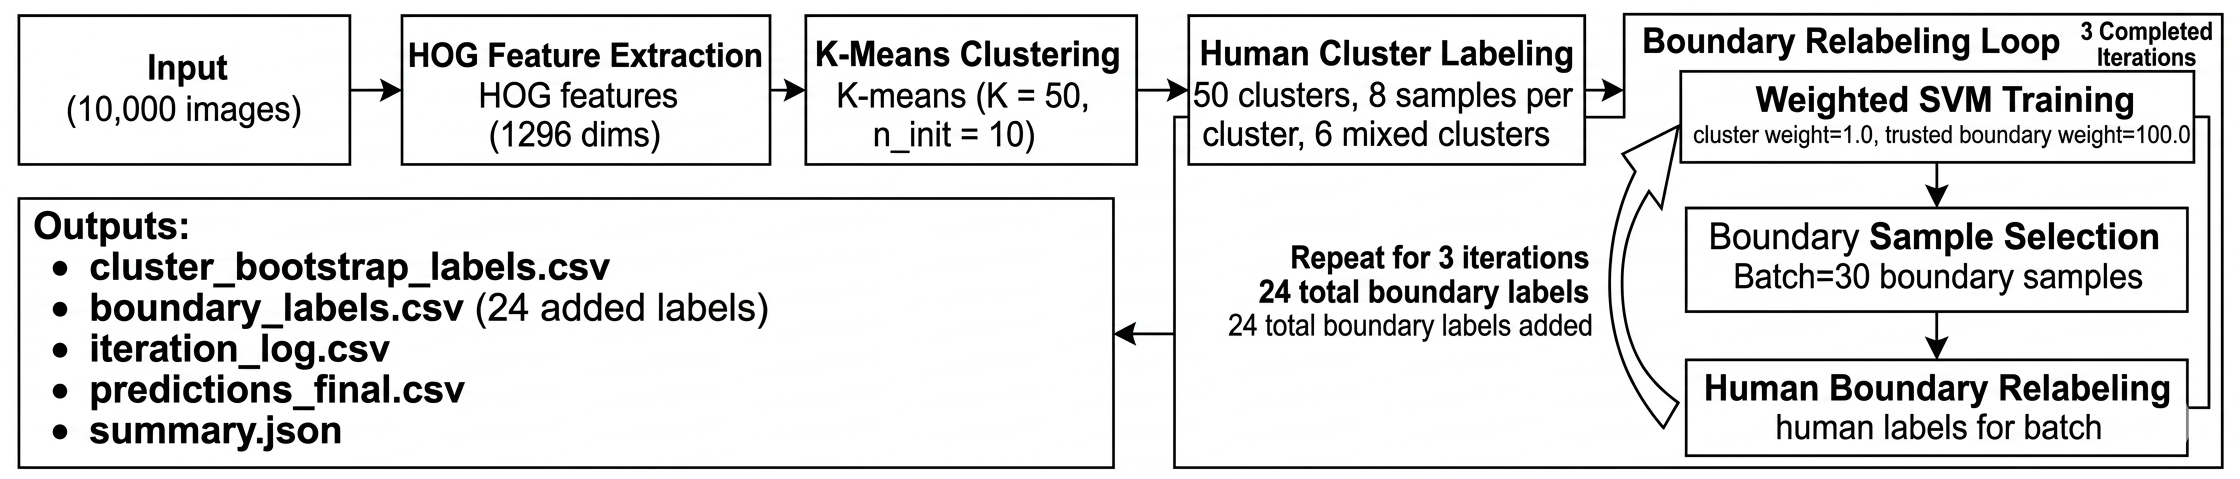
\includegraphics[width=0.96\textwidth]{figures/pipeline1_blockdiagram.png}
\caption{Pipeline 1 block diagram with exact run settings and observed values.}
\label{fig:pipeline1_block}
\end{figure}

\subsubsection{Evaluation and Time Estimate}
Table~\ref{tab:part3_requirements} summarizes the assignment-required metrics from the latest finalized Pipeline 1 run.
\begin{table}[H]
\centering
\caption{Part 3 reporting requirements (compact summary)}
\label{tab:part3_requirements}
\begin{tabular}{p{0.45\textwidth}p{0.48\textwidth}}
\toprule
\textbf{Required Item} & \textbf{Value from Current Run} \\
\midrule
Feature representation (and PCA components if applicable) & HOG, 1296 features (PCA not used) \\
Pipeline 1 exact block diagram with chosen values & Included in Figure~\ref{fig:pipeline1_block} \\
Convergence criterion before oracle test & 500-image practical set; stop when iteration improvement $< 0.1\%$ \\
Number of iterations performed & 3 \\
Last iteration index and train size & Iteration 3, train size = 9210 \\
Boundary labels added in last iteration & 5 \\
Total boundary labels after last iteration & 24 \\
Total manually handled images & 424 images \\
Total estimated manual time & 1240.0 s ($\approx 0.344$ h) \\
Final labeling accuracy (oracle and/or practical) & Oracle: 9909/10000 = 99.09\% \\
\bottomrule
\end{tabular}
\end{table}

\paragraph{Manual effort details.}
From the latest K=50 run (\texttt{run\_20260407\_184753}), the total manual effort is 424 handled images with an estimated 1240.0 seconds ($\approx 0.344$ hours), using the assignment timing model (20 s per cluster decision and 10 s per boundary label).

\paragraph{Accuracy verification.}
The evaluation followed two explicit stages for clarity and assignment compliance:
\begin{itemize}
    \item \textbf{Convergence stage (practical 5\% set):} during iteration, a fixed 500-image human-labeled subset was used to monitor practical measured accuracy. Iteration stops when improvement between consecutive iterations is below 0.1\% (i.e., $\Delta < 0.001$).
        \item \textbf{Final accuracy stage (oracle):} after convergence, final predictions were evaluated against the assignment oracle using \texttt{check\_accuracy.p} in MATLAB Online.
\end{itemize}
The finalized oracle result is 9909 correct out of 10000, giving 99.09\%.

\paragraph{Oracle output evidence (MATLAB Online).}
The following output snippet is from running the oracle check in MATLAB Online:

\begin{lstlisting}[language=Matlab]
>> check

===== Classification Results =====
  Correct : 9909 / 10000
  Accuracy: 99.09%
==================================

accuracy=0.990900
correct=9909/10000
>> 
\end{lstlisting}

\paragraph{MATLAB code used to evaluate \texttt{predictions\_final.csv} with \texttt{check\_accuracy.p}.}
The following reduced MATLAB Online snippet was used to load \texttt{predictions\_final.csv}, validate \texttt{predicted\_label}, and call the P-coded oracle:

\begin{lstlisting}[language=Matlab]
% reduced MATLAB Online checker for predictions_final.csv
T = readtable('predictions_final.csv');

assert(ismember('predicted_label', T.Properties.VariableNames), ...
    'predicted_label column not found');

preds = str2double(string(T.predicted_label));  % handles numeric/text columns
assert(~any(isnan(preds)), ...
    'Found %d missing predicted_label entries.', sum(isnan(preds)));
assert(numel(preds) == 10000, ...
    'predicted vector must have length 10000');

preds_int = int32(preds(:));
try
    [acc, n_correct, n_total] = check_accuracy(preds_int);
    fprintf('accuracy=%.6f\ncorrect=%d/%d\n', acc, n_correct, n_total);
catch
    acc = check_accuracy(preds_int);
    fprintf('accuracy=%g\n', acc);
end
\end{lstlisting}

Part 3 reporting bullets required by the assignment are satisfied for the finalized K=50 run.

\subsubsection{Practical Ground-Truth Convergence Check (5\% Hold-Out)}

A fixed 500-image subset (5\% of the dataset) is manually labeled and used to monitor in-loop convergence without oracle access. The practical subset is used to decide when to stop iterating; the final reported accuracy is still taken from oracle evaluation.

\paragraph{Workflow.}
The single script \texttt{part3/pipline1/pipeline1\_human\_in\_loop.py} supports the full process via practical subcommands:
\begin{itemize}
    \item Prepare a fixed 500-image annotation sheet directly from dataset image IDs (writes CSV with \texttt{image\_id}, blank \texttt{predicted\_label}, and blank \texttt{human\_label}).
    \item Manually fill \texttt{human\_label} (0--9) for all 500 sampled rows.
    \item Run Pipeline 1 with \texttt{--practical-annotated-csv} so each iteration logs practical measured accuracy.
    \item Apply the stopping rule \texttt{--min-improvement 0.001} (0.1\%) and stop when iteration-to-iteration improvement drops below this threshold.
    \item After stopping, evaluate the final \texttt{predictions\_final.csv} with oracle to report the official final accuracy.
\end{itemize}

\begin{table}[H]
\centering
\caption{Additional practical evaluation summary (separate from oracle)}
\label{tab:part3_practical_additional}
\begin{tabular}{>{\raggedright\arraybackslash}p{0.48\textwidth}>{\raggedright\arraybackslash}p{0.42\textwidth}}
\toprule
\textbf{Item} & \textbf{Value} \\
\midrule
Practical hold-out size & 500 images \\
Manual annotation source & Human-labeled subset (5\%) \\
Role of practical subset & In-loop convergence monitoring (stop if improvement $<0.1\%$) \\
Final reported metric & Oracle accuracy on final predictions (99.09\%) \\
\bottomrule
\end{tabular}
\end{table}